
\section{Backend Support}\label{chap:backend}

In this section, we peek inside the Kokkos library and show how a generic parallel for loop is mapped to the OpenMP backend programming model. As a template metaprogramming library, Kokkos makes use of partial specialization. In particular the~\emph{parallel\_for} or ~\emph{parallel\_reduce} function calls, as shown in Figure~\ref{fig:KokkosExample}, are mapped to partially specialized classes. Such classes correspond to a particular backend where for each backend, concepts with partial specialization must be provided. Today, Kokkos supports the CUDA, OpenMP, HIP as well as one-sided MPI, SHMEM and NVSHMEM backends. For each new backend, partially implemented classes that implement necessary concepts must be provided.

A simplified version of a partially specialized class for a parallel for-loop implementation in the OpenMP backend is shown in Figure~\ref{fig:KokkosExampleOMPBackEnd}. The ~\emph{parallel\_for} function instantiates a partial specialization of the ~\emph{ParallelFor} class and calls its ~\emph{execute} function. That function is then responsible to implement the Kokkos parallel pattern. In this backend, the parallel implementation is generated by using OpenMP pragma annotations and a by invoking a compatible compiler when the library is compiled. Figure ~\ref{fig:stack} gives an architectural overview of Kokkos and lists important abstractions as well as the currently supported backends.
\begin{figure}[t!]
\begin{small}
\begin{minted}[fontsize=\small]{c++}
template <class FunctorType>
class ParallelFor<FunctorType,
              RangePolicy<OpenMP>> {
  const FunctorType functor;
  const RangePolicy<OpenMP> policy; 
public:
  void execute() const {
    #pragma omp parallel for
    for(int i=policy.begin();
            i<policy.end();
            ++i)
      functor(i);
  }
};
template <class FunctorType,class PolicyType>
void parallel_for(std::string label, 
    const PolicyType& policy,
    const FunctorType& functor) {
  // Call profiling tool hooks with label
  ParallelFor<FunctorType,PolicyType> 
    pf{functor,policy};
  pf.execute();
}
\end{minted}
\end{small}
\caption{This code shows the backend implementation of a parallel loop in the Kokkos programming model. It shows a particular implementation of a generic pattern as a templated class to the OpenMP execution space. Also, it shows the use of OpenMP pragma annotations that put platform compilers in charge to generate parallel code for the underlying hardware architecture.}
\label{fig:KokkosExampleOMPBackEnd}
\end{figure}

\begin{figure}[t!]
\centerline{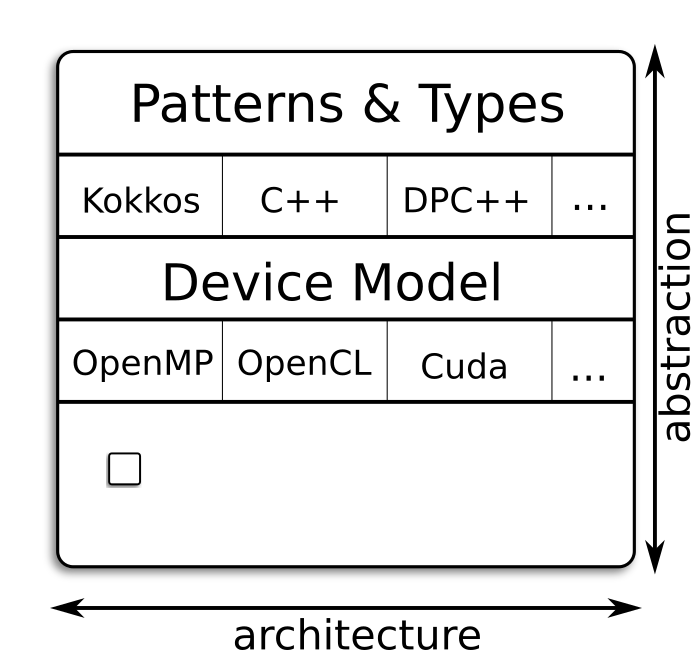
\includegraphics[width=0.42\textwidth]{img/Stack.png}}
\caption{Overview of the Kokkos programming model shows important abstractions as well as the inclusion of backend programming models used by the runtime to map higher level concepts to concrete hardware architectures.}
\label{fig:stack}
\end{figure}

